% Options for packages loaded elsewhere
\PassOptionsToPackage{unicode}{hyperref}
\PassOptionsToPackage{hyphens}{url}
%
\documentclass[
]{article}
\usepackage{lmodern}
\usepackage{amsmath}
\usepackage{ifxetex,ifluatex}
\ifnum 0\ifxetex 1\fi\ifluatex 1\fi=0 % if pdftex
  \usepackage[T1]{fontenc}
  \usepackage[utf8]{inputenc}
  \usepackage{textcomp} % provide euro and other symbols
  \usepackage{amssymb}
\else % if luatex or xetex
  \usepackage{unicode-math}
  \defaultfontfeatures{Scale=MatchLowercase}
  \defaultfontfeatures[\rmfamily]{Ligatures=TeX,Scale=1}
\fi
% Use upquote if available, for straight quotes in verbatim environments
\IfFileExists{upquote.sty}{\usepackage{upquote}}{}
\IfFileExists{microtype.sty}{% use microtype if available
  \usepackage[]{microtype}
  \UseMicrotypeSet[protrusion]{basicmath} % disable protrusion for tt fonts
}{}
\makeatletter
\@ifundefined{KOMAClassName}{% if non-KOMA class
  \IfFileExists{parskip.sty}{%
    \usepackage{parskip}
  }{% else
    \setlength{\parindent}{0pt}
    \setlength{\parskip}{6pt plus 2pt minus 1pt}}
}{% if KOMA class
  \KOMAoptions{parskip=half}}
\makeatother
\usepackage{xcolor}
\IfFileExists{xurl.sty}{\usepackage{xurl}}{} % add URL line breaks if available
\IfFileExists{bookmark.sty}{\usepackage{bookmark}}{\usepackage{hyperref}}
\hypersetup{
  pdftitle={water\_lab\_1},
  hidelinks,
  pdfcreator={LaTeX via pandoc}}
\urlstyle{same} % disable monospaced font for URLs
\usepackage[margin=1in]{geometry}
\usepackage{color}
\usepackage{fancyvrb}
\newcommand{\VerbBar}{|}
\newcommand{\VERB}{\Verb[commandchars=\\\{\}]}
\DefineVerbatimEnvironment{Highlighting}{Verbatim}{commandchars=\\\{\}}
% Add ',fontsize=\small' for more characters per line
\usepackage{framed}
\definecolor{shadecolor}{RGB}{248,248,248}
\newenvironment{Shaded}{\begin{snugshade}}{\end{snugshade}}
\newcommand{\AlertTok}[1]{\textcolor[rgb]{0.94,0.16,0.16}{#1}}
\newcommand{\AnnotationTok}[1]{\textcolor[rgb]{0.56,0.35,0.01}{\textbf{\textit{#1}}}}
\newcommand{\AttributeTok}[1]{\textcolor[rgb]{0.77,0.63,0.00}{#1}}
\newcommand{\BaseNTok}[1]{\textcolor[rgb]{0.00,0.00,0.81}{#1}}
\newcommand{\BuiltInTok}[1]{#1}
\newcommand{\CharTok}[1]{\textcolor[rgb]{0.31,0.60,0.02}{#1}}
\newcommand{\CommentTok}[1]{\textcolor[rgb]{0.56,0.35,0.01}{\textit{#1}}}
\newcommand{\CommentVarTok}[1]{\textcolor[rgb]{0.56,0.35,0.01}{\textbf{\textit{#1}}}}
\newcommand{\ConstantTok}[1]{\textcolor[rgb]{0.00,0.00,0.00}{#1}}
\newcommand{\ControlFlowTok}[1]{\textcolor[rgb]{0.13,0.29,0.53}{\textbf{#1}}}
\newcommand{\DataTypeTok}[1]{\textcolor[rgb]{0.13,0.29,0.53}{#1}}
\newcommand{\DecValTok}[1]{\textcolor[rgb]{0.00,0.00,0.81}{#1}}
\newcommand{\DocumentationTok}[1]{\textcolor[rgb]{0.56,0.35,0.01}{\textbf{\textit{#1}}}}
\newcommand{\ErrorTok}[1]{\textcolor[rgb]{0.64,0.00,0.00}{\textbf{#1}}}
\newcommand{\ExtensionTok}[1]{#1}
\newcommand{\FloatTok}[1]{\textcolor[rgb]{0.00,0.00,0.81}{#1}}
\newcommand{\FunctionTok}[1]{\textcolor[rgb]{0.00,0.00,0.00}{#1}}
\newcommand{\ImportTok}[1]{#1}
\newcommand{\InformationTok}[1]{\textcolor[rgb]{0.56,0.35,0.01}{\textbf{\textit{#1}}}}
\newcommand{\KeywordTok}[1]{\textcolor[rgb]{0.13,0.29,0.53}{\textbf{#1}}}
\newcommand{\NormalTok}[1]{#1}
\newcommand{\OperatorTok}[1]{\textcolor[rgb]{0.81,0.36,0.00}{\textbf{#1}}}
\newcommand{\OtherTok}[1]{\textcolor[rgb]{0.56,0.35,0.01}{#1}}
\newcommand{\PreprocessorTok}[1]{\textcolor[rgb]{0.56,0.35,0.01}{\textit{#1}}}
\newcommand{\RegionMarkerTok}[1]{#1}
\newcommand{\SpecialCharTok}[1]{\textcolor[rgb]{0.00,0.00,0.00}{#1}}
\newcommand{\SpecialStringTok}[1]{\textcolor[rgb]{0.31,0.60,0.02}{#1}}
\newcommand{\StringTok}[1]{\textcolor[rgb]{0.31,0.60,0.02}{#1}}
\newcommand{\VariableTok}[1]{\textcolor[rgb]{0.00,0.00,0.00}{#1}}
\newcommand{\VerbatimStringTok}[1]{\textcolor[rgb]{0.31,0.60,0.02}{#1}}
\newcommand{\WarningTok}[1]{\textcolor[rgb]{0.56,0.35,0.01}{\textbf{\textit{#1}}}}
\usepackage{longtable,booktabs}
\usepackage{calc} % for calculating minipage widths
% Correct order of tables after \paragraph or \subparagraph
\usepackage{etoolbox}
\makeatletter
\patchcmd\longtable{\par}{\if@noskipsec\mbox{}\fi\par}{}{}
\makeatother
% Allow footnotes in longtable head/foot
\IfFileExists{footnotehyper.sty}{\usepackage{footnotehyper}}{\usepackage{footnote}}
\makesavenoteenv{longtable}
\usepackage{graphicx}
\makeatletter
\def\maxwidth{\ifdim\Gin@nat@width>\linewidth\linewidth\else\Gin@nat@width\fi}
\def\maxheight{\ifdim\Gin@nat@height>\textheight\textheight\else\Gin@nat@height\fi}
\makeatother
% Scale images if necessary, so that they will not overflow the page
% margins by default, and it is still possible to overwrite the defaults
% using explicit options in \includegraphics[width, height, ...]{}
\setkeys{Gin}{width=\maxwidth,height=\maxheight,keepaspectratio}
% Set default figure placement to htbp
\makeatletter
\def\fps@figure{htbp}
\makeatother
\setlength{\emergencystretch}{3em} % prevent overfull lines
\providecommand{\tightlist}{%
  \setlength{\itemsep}{0pt}\setlength{\parskip}{0pt}}
\setcounter{secnumdepth}{-\maxdimen} % remove section numbering
\ifluatex
  \usepackage{selnolig}  % disable illegal ligatures
\fi

\title{water\_lab\_1}
\author{}
\date{\vspace{-2.5em}}

\begin{document}
\maketitle

\hypertarget{read-in-data}{%
\subsection{Read-in data}\label{read-in-data}}

Source: USGS Water Quality Portal:
\url{https://www.waterqualitydata.us/}

Site ID: USGS-01646580 Date Range: 01-01-2019 to 03-05-2021

Query:
\url{https://www.waterqualitydata.us/portal/\#siteid=USGS-01646580\&characteristicName=Bicarbonate\&characteristicName=Calcium\&characteristicName=Magnesium\&characteristicName=Sodium\&characteristicName=Potassium\&characteristicName=Hardness\%2C\%20Ca\%2C\%20Mg\&characteristicName=Alkalinity\&characteristicName=pH\&characteristicName=Total\%20dissolved\%20solids\&characteristicName=Temperature\%2C\%20water\&characteristicName=Chloride\&characteristicName=Sulfate\&characteristicName=Carbon\%20dioxide\&startDateLo=01-01-2019\&startDateHi=03-05-2021\&mimeType=csv}

\begin{Shaded}
\begin{Highlighting}[]
\NormalTok{potomac }\OtherTok{\textless{}{-}} \FunctionTok{read\_csv}\NormalTok{(}\StringTok{"data/result\_modified.csv"}\NormalTok{) }\SpecialCharTok{\%\textgreater{}\%} 
  \FunctionTok{mutate}\NormalTok{(}\AttributeTok{Date =} \FunctionTok{as.Date}\NormalTok{(Date, }\StringTok{"\%m/\%d/\%Y"}\NormalTok{))}
\end{Highlighting}
\end{Shaded}

\begin{verbatim}
## 
## -- Column specification --------------------------------------------------------------------------------------------------------------------------
## cols(
##   ID = col_character(),
##   Date = col_character(),
##   Location_ID = col_character(),
##   Hydrologic = col_character(),
##   Parameter = col_character(),
##   Fraction = col_character(),
##   Value = col_double(),
##   Units = col_character(),
##   Method_name = col_character(),
##   Method_source = col_character()
## )
\end{verbatim}

\hypertarget{inspect-data}{%
\subsection{Inspect Data}\label{inspect-data}}

\begin{Shaded}
\begin{Highlighting}[]
\CommentTok{\# Bar chart of \# of parameters analyzed by date}

\NormalTok{potomac }\SpecialCharTok{\%\textgreater{}\%} 
  \FunctionTok{ggplot}\NormalTok{(}\FunctionTok{aes}\NormalTok{(}\AttributeTok{x =}\NormalTok{ Date)) }\SpecialCharTok{+}
    \FunctionTok{geom\_bar}\NormalTok{(}\AttributeTok{stat =} \StringTok{"count"}\NormalTok{) }\SpecialCharTok{+}
  \FunctionTok{theme\_bw}\NormalTok{()}
\end{Highlighting}
\end{Shaded}

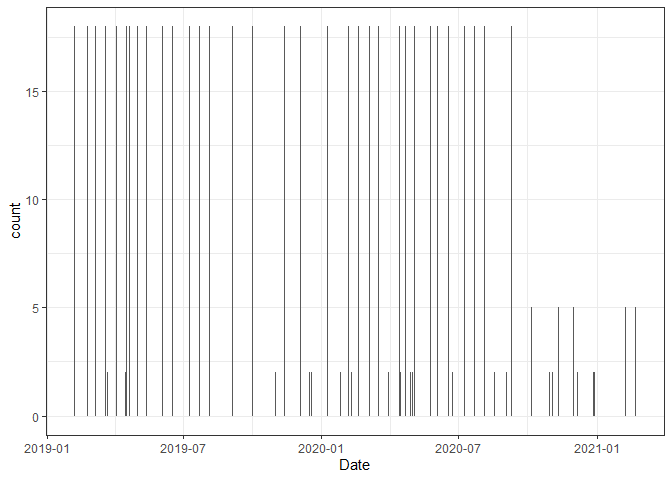
\includegraphics{water_lab_1_files/figure-latex/unnamed-chunk-2-1.pdf}

\begin{Shaded}
\begin{Highlighting}[]
\CommentTok{\# Summary table of parameter values}

\NormalTok{potomac }\SpecialCharTok{\%\textgreater{}\%} 
  \FunctionTok{group\_by}\NormalTok{(Parameter) }\SpecialCharTok{\%\textgreater{}\%} 
    \FunctionTok{summarise}\NormalTok{(}\AttributeTok{mean =} \FunctionTok{round}\NormalTok{(}\FunctionTok{mean}\NormalTok{(Value), }\AttributeTok{digits =} \DecValTok{2}\NormalTok{),}
              \AttributeTok{sd =} \FunctionTok{round}\NormalTok{(}\FunctionTok{sd}\NormalTok{(Value), }\AttributeTok{digits =} \DecValTok{2}\NormalTok{),}
              \AttributeTok{upper95 =} \FunctionTok{round}\NormalTok{(}\FunctionTok{quantile}\NormalTok{(Value, .}\DecValTok{95}\NormalTok{), }\AttributeTok{digits =} \DecValTok{2}\NormalTok{),}
              \AttributeTok{n =} \FunctionTok{n}\NormalTok{()) }\SpecialCharTok{\%\textgreater{}\%} 
\NormalTok{  knitr}\SpecialCharTok{::}\FunctionTok{kable}\NormalTok{()}
\end{Highlighting}
\end{Shaded}

\begin{verbatim}
## `summarise()` ungrouping output (override with `.groups` argument)
\end{verbatim}

\begin{longtable}[]{@{}lrrrr@{}}
\toprule
Parameter & mean & sd & upper95 & n\tabularnewline
\midrule
\endhead
Alkalinity & 91.30 & 17.81 & 118.50 & 71\tabularnewline
Bicarbonate & 109.37 & 21.21 & 139.30 & 38\tabularnewline
Calcium & 34.18 & 6.05 & 42.96 & 33\tabularnewline
Carbon dioxide & 1.70 & 0.85 & 3.20 & 38\tabularnewline
Chloride & 16.88 & 5.33 & 25.02 & 33\tabularnewline
Hardness, Ca, Mg & 120.73 & 23.83 & 159.60 & 33\tabularnewline
Magnesium & 8.53 & 2.30 & 12.36 & 33\tabularnewline
pH & 8.09 & 0.24 & 8.40 & 90\tabularnewline
Potassium & 2.32 & 0.58 & 3.30 & 33\tabularnewline
Sodium & 9.94 & 2.29 & 13.76 & 33\tabularnewline
Sulfate & 24.05 & 6.30 & 36.22 & 33\tabularnewline
Temperature, water & 14.52 & 8.72 & 29.10 & 57\tabularnewline
Total dissolved solids & 1688.75 & 4003.64 & 8047.00 &
132\tabularnewline
\bottomrule
\end{longtable}

\begin{Shaded}
\begin{Highlighting}[]
\CommentTok{\# Boxplot of Parameter Values}

\NormalTok{potomac }\SpecialCharTok{\%\textgreater{}\%} 
  \FunctionTok{filter}\NormalTok{(}\SpecialCharTok{!}\NormalTok{Parameter }\SpecialCharTok{\%in\%} \FunctionTok{c}\NormalTok{(}\StringTok{"Total dissolved solids"}\NormalTok{,}
                           \StringTok{"Temperature, water"}\NormalTok{, }\StringTok{"pH"}\NormalTok{, }\StringTok{"Hardness, Ca, Mg"}\NormalTok{,}
                           \StringTok{"Alkalinity"}\NormalTok{)) }\SpecialCharTok{\%\textgreater{}\%} 
  \FunctionTok{ggplot}\NormalTok{(}\FunctionTok{aes}\NormalTok{(}\AttributeTok{x =}\NormalTok{ Parameter, }\AttributeTok{y =}\NormalTok{ Value)) }\SpecialCharTok{+}
    \FunctionTok{geom\_boxplot}\NormalTok{() }\SpecialCharTok{+}
    \FunctionTok{coord\_flip}\NormalTok{() }\SpecialCharTok{+}
    \FunctionTok{ylab}\NormalTok{(}\StringTok{"mg/L"}\NormalTok{) }\SpecialCharTok{+}
    \FunctionTok{ggtitle}\NormalTok{(}\StringTok{"Ions"}\NormalTok{) }\SpecialCharTok{+}
    \FunctionTok{theme\_bw}\NormalTok{()}
\end{Highlighting}
\end{Shaded}

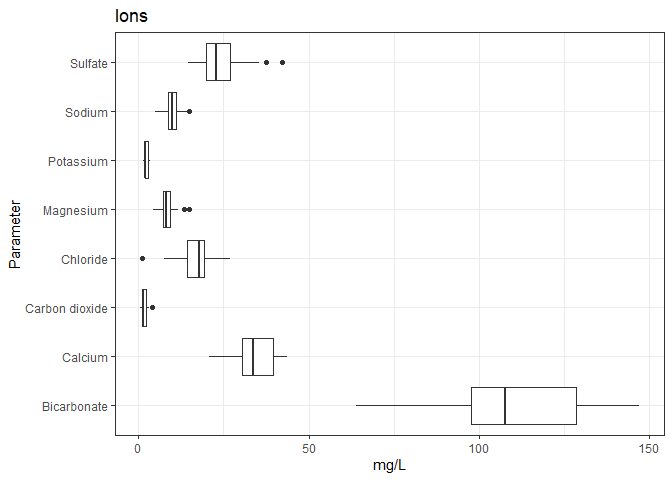
\includegraphics{water_lab_1_files/figure-latex/unnamed-chunk-2-2.pdf}

\begin{Shaded}
\begin{Highlighting}[]
\NormalTok{potomac }\SpecialCharTok{\%\textgreater{}\%} 
  \FunctionTok{filter}\NormalTok{(Parameter }\SpecialCharTok{\%in\%} \FunctionTok{c}\NormalTok{(}\StringTok{"Hardness, Ca, Mg"}\NormalTok{, }\StringTok{"Alkalinity"}\NormalTok{)) }\SpecialCharTok{\%\textgreater{}\%} 
  \FunctionTok{ggplot}\NormalTok{(}\FunctionTok{aes}\NormalTok{(}\AttributeTok{x =}\NormalTok{ Parameter, }\AttributeTok{y =}\NormalTok{ Value)) }\SpecialCharTok{+}
    \FunctionTok{geom\_boxplot}\NormalTok{() }\SpecialCharTok{+}
    \FunctionTok{coord\_flip}\NormalTok{() }\SpecialCharTok{+}
    \FunctionTok{ylab}\NormalTok{(}\FunctionTok{expression}\NormalTok{(}\StringTok{"mg/L as CaCO"}\NormalTok{[}\DecValTok{3}\NormalTok{])) }\SpecialCharTok{+}
    \FunctionTok{ggtitle}\NormalTok{(}\StringTok{"Hardness and Alkalinity"}\NormalTok{) }\SpecialCharTok{+}
    \FunctionTok{theme\_bw}\NormalTok{()}
\end{Highlighting}
\end{Shaded}

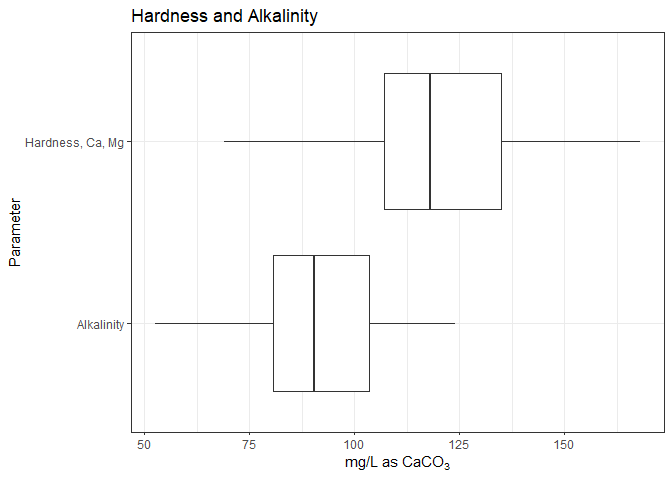
\includegraphics{water_lab_1_files/figure-latex/unnamed-chunk-2-3.pdf}

\begin{Shaded}
\begin{Highlighting}[]
\NormalTok{potomac }\SpecialCharTok{\%\textgreater{}\%} 
  \FunctionTok{filter}\NormalTok{(Parameter }\SpecialCharTok{\%in\%} \StringTok{"pH"}\NormalTok{) }\SpecialCharTok{\%\textgreater{}\%} 
  \FunctionTok{ggplot}\NormalTok{(}\FunctionTok{aes}\NormalTok{(}\AttributeTok{x =}\NormalTok{ Parameter, }\AttributeTok{y =}\NormalTok{ Value)) }\SpecialCharTok{+}
    \FunctionTok{geom\_boxplot}\NormalTok{() }\SpecialCharTok{+}
    \FunctionTok{coord\_flip}\NormalTok{() }\SpecialCharTok{+}
    \FunctionTok{ylab}\NormalTok{(}\StringTok{"pH"}\NormalTok{) }\SpecialCharTok{+}
    \FunctionTok{ggtitle}\NormalTok{(}\StringTok{"pH"}\NormalTok{) }\SpecialCharTok{+}
    \FunctionTok{theme\_bw}\NormalTok{()}
\end{Highlighting}
\end{Shaded}

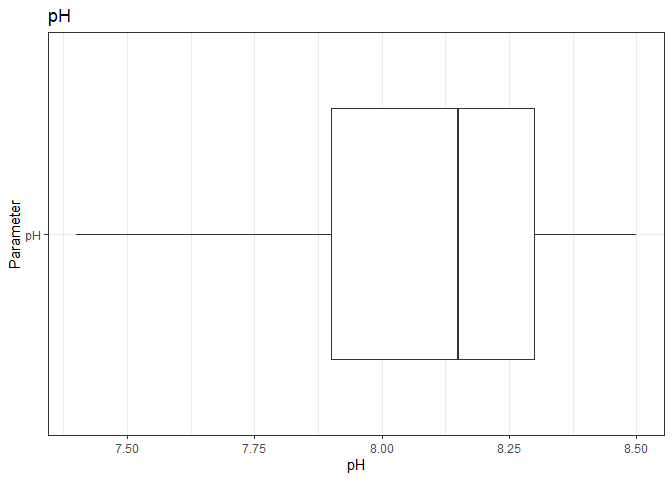
\includegraphics{water_lab_1_files/figure-latex/unnamed-chunk-2-4.pdf}

\hypertarget{select-data}{%
\subsection{Select data}\label{select-data}}

Filter most recent results with full set of parameter results

\begin{Shaded}
\begin{Highlighting}[]
\NormalTok{potomac }\SpecialCharTok{\%\textgreater{}\%} 
  \FunctionTok{group\_by}\NormalTok{(Date) }\SpecialCharTok{\%\textgreater{}\%}
    \FunctionTok{count}\NormalTok{() }\SpecialCharTok{\%\textgreater{}\%} 
    \FunctionTok{arrange}\NormalTok{(}\FunctionTok{desc}\NormalTok{(Date)) }\SpecialCharTok{\%\textgreater{}\%} 
  \FunctionTok{View}\NormalTok{()}
\end{Highlighting}
\end{Shaded}

2020-09-10: most recent sample day with 18 parameters

\begin{Shaded}
\begin{Highlighting}[]
\NormalTok{potomac }\SpecialCharTok{\%\textgreater{}\%} 
  \FunctionTok{filter}\NormalTok{(Date }\SpecialCharTok{==} \StringTok{"2020{-}09{-}10"}\NormalTok{)}
\end{Highlighting}
\end{Shaded}

\begin{verbatim}
## # A tibble: 18 x 10
##    ID           Date       Location_ID   Hydrologic   Parameter        Fraction   Value Units   Method_name           Method_source               
##    <chr>        <date>     <chr>         <chr>        <chr>            <chr>      <dbl> <chr>   <chr>                 <chr>                       
##  1 nwismd.01.0~ 2020-09-10 USGS-01646580 Falling sta~ Temperature, wa~ <NA>       25.5  deg C   Temperature, water, ~ USGS National Field Manual,~
##  2 nwismd.01.0~ 2020-09-10 USGS-01646580 Falling sta~ pH               Total       8.2  std un~ pH, field, electrome~ USGS National Field Manual,~
##  3 nwismd.01.0~ 2020-09-10 USGS-01646580 Falling sta~ pH               Total       8.2  std un~ pH, lab, auto glass ~ USGS TWRI 5-A1/1989, p 363  
##  4 nwismd.01.0~ 2020-09-10 USGS-01646580 Falling sta~ Carbon dioxide   Total       1.2  mg/l    Computation by NWIS ~ NWIS User's Manual, QW Syst~
##  5 nwismd.01.0~ 2020-09-10 USGS-01646580 Falling sta~ Bicarbonate      Dissolv~  115    mg/l    Alkalinity, IPT, Hac~ Rounds, 2007, Alkalinity ca~
##  6 nwismd.01.0~ 2020-09-10 USGS-01646580 Falling sta~ Hardness, Ca, Mg <NA>      125    mg/l C~ Computation by NWIS ~ NWIS User's Manual, QW Syst~
##  7 nwismd.01.0~ 2020-09-10 USGS-01646580 Falling sta~ Calcium          Dissolv~   35.5  mg/l    Metals, wf, ICP-AES ~ USGS OF 93-125, p 101       
##  8 nwismd.01.0~ 2020-09-10 USGS-01646580 Falling sta~ Magnesium        Dissolv~    8.72 mg/l    Metals, wf, ICP-AES ~ USGS OF 93-125, p 101       
##  9 nwismd.01.0~ 2020-09-10 USGS-01646580 Falling sta~ Sodium           Dissolv~    8.92 mg/l    Metals, wf, ICP-AES ~ USGS OF 93-125, p 101       
## 10 nwismd.01.0~ 2020-09-10 USGS-01646580 Falling sta~ Potassium        Dissolv~    2.69 mg/l    Potassium, wf, by IC~ Standard Methods            
## 11 nwismd.01.0~ 2020-09-10 USGS-01646580 Falling sta~ Chloride         Dissolv~   14.3  mg/l    Anions, wf, IC        Standard Methods (22d ed), ~
## 12 nwismd.01.0~ 2020-09-10 USGS-01646580 Falling sta~ Sulfate          Dissolv~   28.4  mg/l    Anions, wf, IC        Standard Methods (22d ed), ~
## 13 nwismd.01.0~ 2020-09-10 USGS-01646580 Falling sta~ Alkalinity       Dissolv~   96.5  mg/l C~ Alkalinity, titr. pH~ USGS TWRI 5-A1/1989, p 57   
## 14 nwismd.01.0~ 2020-09-10 USGS-01646580 Falling sta~ Alkalinity       Dissolv~   95.3  mg/l C~ Alkalinity, IPT, Hach USGS National Field Manual  
## 15 nwismd.01.0~ 2020-09-10 USGS-01646580 Falling sta~ Total dissolved~ Dissolv~  168    mg/l    ROE, wf, 180C, by we~ USGS TWRI 5-A1/1989, p 437  
## 16 nwismd.01.0~ 2020-09-10 USGS-01646580 Falling sta~ Total dissolved~ Dissolv~  166    mg/l    Computation by NWIS ~ NWIS User's Manual, QW Syst~
## 17 nwismd.01.0~ 2020-09-10 USGS-01646580 Falling sta~ Total dissolved~ Dissolv~ 2510    tons/d~ Computation by NWIS ~ NWIS User's Manual, QW Syst~
## 18 nwismd.01.0~ 2020-09-10 USGS-01646580 Falling sta~ Total dissolved~ Dissolv~    0.23 tons/a~ Computation by NWIS ~ NWIS User's Manual, QW Syst~
\end{verbatim}

\begin{Shaded}
\begin{Highlighting}[]
\NormalTok{potomac }\SpecialCharTok{\%\textgreater{}\%} 
  \FunctionTok{filter}\NormalTok{(Date }\SpecialCharTok{==} \StringTok{"2020{-}09{-}10"}\NormalTok{) }\SpecialCharTok{\%\textgreater{}\%} 
\NormalTok{  dplyr}\SpecialCharTok{::}\FunctionTok{select}\NormalTok{(Parameter, Value, Units) }\SpecialCharTok{\%\textgreater{}\%} 
\NormalTok{  knitr}\SpecialCharTok{::}\FunctionTok{kable}\NormalTok{()}
\end{Highlighting}
\end{Shaded}

\begin{longtable}[]{@{}lrl@{}}
\toprule
Parameter & Value & Units\tabularnewline
\midrule
\endhead
Temperature, water & 25.50 & deg C\tabularnewline
pH & 8.20 & std units\tabularnewline
pH & 8.20 & std units\tabularnewline
Carbon dioxide & 1.20 & mg/l\tabularnewline
Bicarbonate & 115.00 & mg/l\tabularnewline
Hardness, Ca, Mg & 125.00 & mg/l CaCO3\tabularnewline
Calcium & 35.50 & mg/l\tabularnewline
Magnesium & 8.72 & mg/l\tabularnewline
Sodium & 8.92 & mg/l\tabularnewline
Potassium & 2.69 & mg/l\tabularnewline
Chloride & 14.30 & mg/l\tabularnewline
Sulfate & 28.40 & mg/l\tabularnewline
Alkalinity & 96.50 & mg/l CaCO3\tabularnewline
Alkalinity & 95.30 & mg/l CaCO3\tabularnewline
Total dissolved solids & 168.00 & mg/l\tabularnewline
Total dissolved solids & 166.00 & mg/l\tabularnewline
Total dissolved solids & 2510.00 & tons/day\tabularnewline
Total dissolved solids & 0.23 & tons/ac ft\tabularnewline
\bottomrule
\end{longtable}

\end{document}
